\section{Description of Datasets}
\label{sec:methods/section_a}

To our knowledge, there is no public or open-source dataset of uncompressed video sequences with object tracking ground truth. Our group members prepared the uncompressed HEVC v1 Common Test Conditions (CTC) sequences \cite{bossen_common_2013} in the YUV420 format. The dataset can be obtained from Joint Collaborative Team on Video Coding (JCT-VC). They annotated them to obtain object detection ground truth, using YOLOv3 \cite{redmon_yolov3_2018} and YOLO Mark software \cite{alexey_alexeyabyolo_mark_2021} as the semi-automated annotation process \cite{choi_dataset_2021}. The existing annotations prepared by our group members are suitable for object detection; however, for the purpose of analyzing the tracking performance, we further annotated the unique object identifier (ID) on the existing ground truths using Normalized Cross-correlation (NCC) \cite{zhao_image_2006}. NCC value gives a similarity between two images. Figure \ref{fig:annotation} shows the semi-automated annotation procedure for assigning unique IDs.
\begin{figure}[!tb]
  \centering
  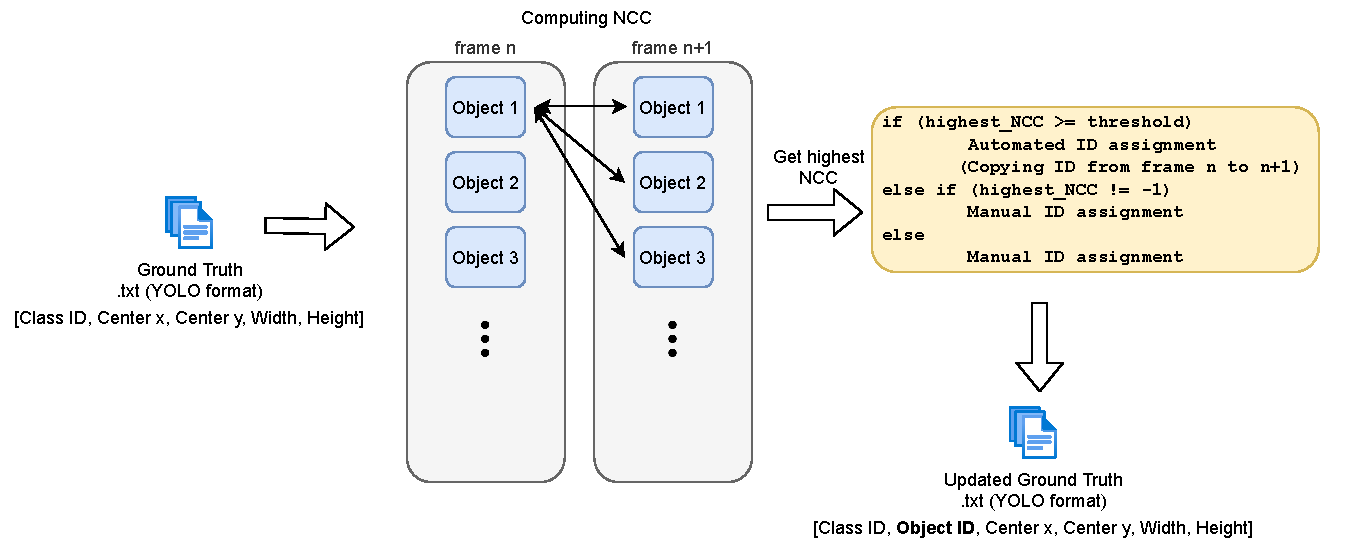
\includegraphics[width=1.0\linewidth]{img/annotation.pdf}
  \caption[Semi-automated annotation process for ID assignment in the ground truth]
  {Semi-automated annotation process for ID assignment in the ground truth.}
  \label{fig:annotation}
\end{figure}
Given the existing ground truth, each object annotation is in the YOLO format as [Class ID, Center x, Center y, Width, Height, Confidence]. Class ID indicates the identifier to the type of object class; for example, "person" as 0, "sports ball" as 32, and "chair" as 56, which are part of the 80 COCO object classes \cite{lin_microsoft_2014}. Center x and Center y are the center position of the bounding box in relative coordinates\footnote{A value in a relative coordinate is equivalent to a value in a pixel coordinate divided by the frame width horizontally and the frame height vertically.}; Width and Height are the corresponding dimensions of boxes in relative coordinates. We compare every object in the previous frame $n$ with the current frame $n+1$ and compute NCC values for every possible pair between those image patches of objects. As shown in the pseudocode in Figure \ref{fig:annotation}, we take the pair of objects that corresponds to the highest NCC value, and if the value is greater than or equal to the threshold, we assign an unique ID automatically according to the pair. Threshold is a value that tells how confident the two image patches of objects are similar, and we chose 0.60 for most video sequences. If the highest NCC is less than the threshold, ID is manually assigned. When there is no pair of objects between the previous and current frame, the highest NCC is assigned -1 to signal that the pair of objects does not exist, and ID is manually assigned. This situation could happen when objects do not exist for the particular object class in the previous frame but objects exist in the current frame. Throughout this semi-automated process of annotation, object IDs are assigned in the second column of ground truth files.
\begin{table}[htb]
    \centering
    \caption{List of Video Sequences adapted from \cite{choi_vcm_2020}}
    \resizebox{1.0\linewidth}{!}{
    \begin{tabular}{|| c | c | c | c | c | c | c ||}
         \hline
          Sequence Class & Sequence Name & Frame Count & Resolution & Object Class IDs & Frame rate (Hz) & Bit depth  \\ [0.5ex]
         \hline\hline
          B & BasketballDrive & 500 & 1920x1080 & [0, 32, 56] & 50 & 8 \\ 
         \hline
          B & Cactus & 500 & 1920x1080 & [58] & 50 & 8 \\ 
         \hline
          B & Kimono & 240 & 1920x1080 & [0, 26] & 24 & 8 \\
         \hline
          B & ParkScene & 240 & 1920x1080 & [0, 1, 13] & 24 & 8 \\
         \hline
          C & BasketballDrill & 500 & 832x480 & [0, 32, 56] & 50 & 8 \\
         \hline
          C & PartyScene & 500 & 832x480 & [0, 41, 58, 74, 77] & 50 & 8 \\
         \hline
          C & RaceHorses & 300 & 832x480 & [0, 17] & 30 & 8 \\
         \hline
          D & BasketballPass & 500 & 416x240 & [0, 32, 56] & 50 & 8 \\
         \hline
          D & BlowingBubbles & 500 & 416x240 & [0, 41, 77] & 50 & 8 \\
          \hline
          D & RaceHorses & 500 & 416x240 & [0, 17] & 30 & 8 \\
          \hline
          E & KristenAndSara & 600 & 1280x720 & [0, 63, 67] & 60 & 8 \\
          \hline
          E & Johnny & 600 & 1280x720 & [0, 27, 63] & 60 & 8 \\
          \hline
          E & FourPeople & 600 & 1280x720 & [0, 41, 56, 58] & 60 & 8 \\
          \hline
    \end{tabular}
    }
    \label{tab:seq_list}
\end{table}
Table \ref{tab:seq_list} shows the 13 uncompressed HEVC v1 CTC video sequences for which we created ground truth annotations, out of 18 available video sequences from \cite{choi_dataset_2021}. The sequence class (B, C, D, E) indicates the resolution ($\text{Width} \times \text{Height}$). Each sequence has different number of object classes and each class ID is from the 80 COCO object classes \cite{lin_microsoft_2014}. Table \ref{tab:class_id}, adapted from \cite{choi_dataset_2021}, shows the corresponding object class name for each class ID, and we only listed the object classes that we detect and track in the given sequences from Table \ref{tab:seq_list}.
\begin{table}[!htbp]
    \centering
    \caption{List of Object Class IDs adapted from \cite{choi_vcm_2020}}
    \resizebox{0.6\linewidth}{!}{
    \begin{tabular}{|| c | c | c | c ||}
         \hline
          Class ID & Object class name & Class ID & Object class name \\ [0.5ex]
         \hline\hline
          0 & Person & 41 & Cup \\
         \hline
          1 & Bicycle & 56 & Chair \\
         \hline
         13 & Bench & 58 & Potted plant \\
         \hline
         17 & Horse & 63 & Laptop \\
         \hline
         26 & Handbag & 67 & Cell phone \\
         \hline
         27 & Tie & 74 & Clock \\
         \hline
         32 & Sports ball & 77 & Teddy bear \\
         \hline
    \end{tabular}
    }
    \label{tab:class_id}
\end{table}
In the experiments, "all" refers to all object classes available in the ground truth. The object tracking pipeline consists of the YOLOv3 detector and SORT, as shown in Figure \ref{fig:yolov3+SORT}. 
\begin{figure}[!htbp]
  \centering
  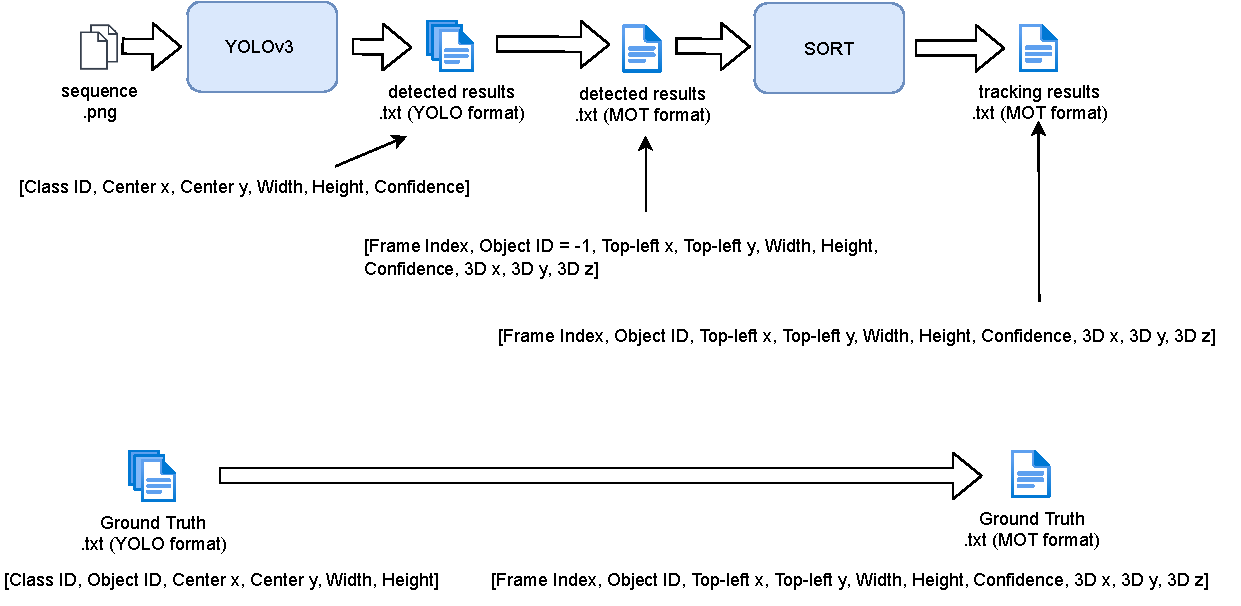
\includegraphics[width=1.0\linewidth]{img/YOLOv3+SORT.pdf}
  \caption[Object tracking pipeline with YOLO v3 and SORT]
  {Object tracking pipeline with YOLO v3 and SORT.}
  \label{fig:yolov3+SORT}
\end{figure}
Input video sequences of PNG files are input to the YOLOv3 object detector. The output from YOLOv3 will be generated in the YOLO format as [Class ID, Center x, Center y, Width, Height, Confidence]. Note that Confidence is the object class probability, and this score tells how confident the object is detected for the particular class. These results are converted to the MOT format used in the MOT Challenge 2015 benchmark \cite{leal-taixe_motchallenge_2015}. The object ID, the unique identifier to the object, for the detected result is initialized as -1. Applying SORT to this detected result, we obtain the tracking result in the MOT format with the assigned object ID as [Frame index, Object ID, Top-left x, Top-left y, Width, Height, Confidence, 3D x, 3D y, 3D z]. Top-left x and Top-left y are the positions of the bounding box at the top-left corner in pixel coordinates. Width and Height are dimensions of boxes in pixel coordinates. 3D x, 3D y, 3D z are the bounding box position in 3D, but we assigned -1 in our experiment since the 3D position is not applicable to our experiment. The ground truth is also converted from the YOLO format to the MOT format.

% The MOT format from \textit{MOTChallenge} is summarized in 
% \begin{myfont}
% \centering
% Class ID, Object ID, center X, center Y, Width, Height
% \end{myfont}


% \begin{table}[]
%     \centering
%     \caption{}
%     \begin{tabular}{|c|c|}
%         \hline
%         Data field & Description \\
%         \hline\hline
%         Frame Index & Frame index in a sequence \\
%         \hline
%         Object ID & Unique identifier to the object \\
%         \hline
%         Top-left x & x coordinate in top-left corner of the bounding box \\
%         \hline
%         Top-left y & y coordinate in top-left corner of the bounding box \\
%         \hline
%         Width & Width of the bounding box \\
%         \hline
%         Height & Height of the bounding box \\
%         \hline
%         Confidence & Confidence score of the detection of the object \\
%         \hline
%         3D x & x coordinate in 3D bounding box \\
%         \hline
%         3D y & y coordinate in 3D bounding box \\
%         \hline
%         3D z & z coordinate in 3D bounding box \\
%         \hline
%     \end{tabular}
%     \label{tab:MOT_format}
% \end{table}


